\documentclass[output=paper]{LSP/langsci} 
\ChapterDOI{10.5281/zenodo.1090948}
\title{The influence of self-monitoring on the translation of cognates}
\author{Katharina Oster}
\affiliation{Johannes-Gutenberg-Universität Mainz}
\abstract{In some translations, the source text influences the syntactic structures or the lexis of the target text (shining-through), while other translations contain fewer traces of  language transfer than original texts in the target language (normalization). On the lexical level, this can be seen in the number of cognates. There is no definite answer to the question of how these phenomena can be linked to mental processes yet. However, psycholinguistic literature shows that the shining-through effect can be explained by the structure of the mental lexicon as well as the mechanisms for accessing words: the cognate-facilitation-effect. The aim of this study is to provide an explanation for normalization. The hypothesis was that verbal self-monitoring, after the first activation of words but before articulation, filters out cognates. For this purpose, written and oral translations were compared. Written translations, which are monitored more strongly, contained fewer cognates than oral translations. Accordingly, the interpretation of this study was that self-monitoring filters out cognates before the translator starts writing and that it is therefore an important factor for normalization.}

\maketitle
\begin{document}

\section{Introduction}\label{oster:sec:1}
Translations differ from original texts. In some translations, the influence of the source text on syntactic structures or the lexis of the target text is visible (shining through; \citealt{Teich2003}) while other translations contain fewer traces of language transfer than original texts in the \isi{target language} -- the translator seems to exagerate the norms of the \isi{target language} (normalization; \citealt{Baker1996}). So far, we do not know the exact mental causes of these phenomena. This study is therefore an attempt to find answers to this question. 

\subsection{Cognates, shining through and normalization}\label{oster:sec:1.1}
Cognates are words which share both form and meaning in the source and target languages -- e.g.\ the English word \textit{system} and the \ili{German} word \textit{System} \citep{Stamenov2010}. In corpus linguistics, cognates have been used to identify normalization and shining-through on the lexical level: in comparison to the originals, shining through can be observed in the use of more cognates and normalization in the use of fewer cognates --  provided that language preserving tendencies exist in the respective language (e.g. in \ili{Slovene} -- \citealt{Vintar2005}). 

Several external factors can lead to normalization or shining-through in translations. These include, for example, the language pair but also the text type: the language pair English-\ili{German}, for example, has been shown to be quite prone to shining-through while the language pair English-\ili{Slovene} leans towards normalization \citep{Vintar2005}.

Shining-through and normalization are especially interesting with regard to the question of how translators deal with language contact and language control in their mind. These processes might not only be interesting in regard to translations but also in terms of language change. Although there may be other factors that influence languages such as \ili{German} for example \citet{HansenSchirra2012What}, a study by \citet{Becher2009Convergence} suggests that translations have an influence on the lexical features in the \isi{target language}. Understanding the mental mechanisms that result in shining-through and normalization is therefore not only interesting with regard to modeling the \isi{translation process} but also when it comes to understanding how the human mind can cause and control language changes.

\subsection{The translation process}\label{oster:sec:1.2}
Different models have been proposed to describe the mental processes during translation. However, many models in the field of translation studies do not concentrate on pure language processing but on other factors, such as problem solving and the integration of different types of information (e.g. \citealt{Honig1997}, \citealt{Kiraly1995Pathways}, \citealt{Krings1986Was}). Other models are very simple and do not integrate different language processing steps, such as the processing of words (e.g. \citealt{Kautz2000}, \citealt{Steiner2001Translations}). These models can therefore not be used to explain the processing of cognates during translation. For the purpose of the present study, I will thus suggest a model that concentrates on the mental processing of words during translation.

In the field of psycholinguistics, many researchers have presented speech process models that concentrate on the processing of words. \citet{Levelt1989} described one of the first complete speech process models which served as a foundation for further monolingual and bilingual models \citep{DeGroot2011}. He distinguishes between a reception and a production phase. During reception, a person hears spoken speech or reads a text. During comprehension, he then maps phonological and orthographical information to lexical entries and grammatical information stored in his long term memory. He finally accesses meaning by linking this linguistic information to abstract concepts. During production, a speaker first creates a preverbal message. He chooses, for example, the overall idea, the perspective and the language of his message. In Levelt's model, this step is called conceptualization. The speaker then accesses lexical entries, morphology and grammatical structures during the formulation phase in order to give his message a verbal structure. The stage during which all linguistic information necessary for producing speech is accessed is called \textit{inner speech}. The final step is the physical act of speaking or writing.

Levelt's model has been modified by many researchers (for reviews see \citealt{DeGroot2011}; \citealt{Plieger2006}). Several components have been added in order to make it suitable for \isi{bilinguals} and for interaction with other speakers. It has also been discussed in which order the components are accessed and whether the process is only top-down, like in Levelt's model, or whether the different stages might interact, occur more or less simultaneously and whether the conceptual level might be influenced by the language chosen for production \citep{Dell1992}. But most complete speech process models contain the five steps listed above: hearing, comprehension, conceptualization, formulation and speaking (cf. \citealt{Plieger2006}).

Levelt's model could also be a good foundation for a \isi{translation process model}. \citet{Kautz2000} and \citet{Steiner2001Translations}, for example, also divided their \isi{translation process} models into a reception and a production phase. And even though some researchers argue that translators do not always access meaning (the conceptual level, cf. \citealt{DeGroot2011}), but instead sometimes just transcribe messages, some studies (e.g. \citealt{Francis2005}) have given reason to believe that translators always pass through the different steps described above and access the conceptual level.

For the purpose of this study, I suggest the \isi{translation process model} in \figref{oster:fig:1} which is based on Levelt's model and which assumes that translators always access meaning. Translators read the text, then link the orthographical and phonological information to lexical and grammatical information, and access meaning. Next, translators might change the message before they choose lexical and grammatical information in the \isi{target language} in order to verbalize the message. They finally articulate the message or write it down. This model does not aim to explain all language processing steps during translation or how the translator deals with information during conceptualization, but rather seeks to locate the processing of words during translation because this is the step which could be responsible for shining-through and normalization. In the model proposed in \figref{oster:fig:1}, the translator accesses words in the \isi{mental lexicon} during the comprehension phase (reception) and during the formulation phase (production) (see also \citealt{Levelt1989}). Although, the different steps are clear cut and unidirectional in \figref{oster:fig:1}, we must assume that there is interaction between the different components and that the different processing steps might overlap or take place simultaneously.

\begin{figure}	
    \resizebox{.5\textwidth}{!}{
    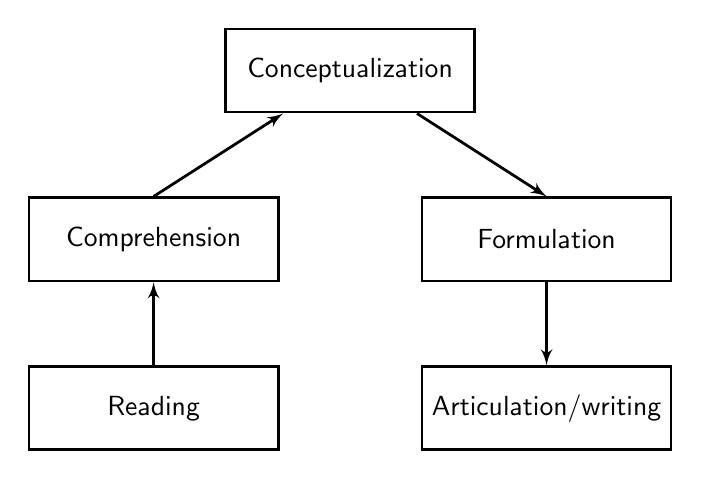
\begin{tikzpicture}
        \usetikzlibrary{shapes,arrows,positioning}
    % Define Styles
        \tikzstyle{block} = [rectangle, draw, fill=white, text centered, minimum height=3em, minimum width = 9em, line width = 0.1em]
        \tikzstyle{line} = [draw, -latex', line width=0.1em]
        \tikzstyle{block} = [rectangle, draw, fill=white, text centered, minimum height=3em, minimum width = 9em, line width = 0.1em]
        \tikzstyle{line} = [draw, -latex', line width=0.1em]
    % Place nodes
        \node [block] (conceptualization) {\sffamily{Conceptualization}};
        \node [block, below left = 3em and -2em  of conceptualization] (comprehension) {\sffamily{Comprehension}};
        \node [block, below right = 3em and -2em of conceptualization] (formulation) {\sffamily{Formulation}};
        \node [block, below = 3em of formulation] (articulation) {\sffamily{Articulation/writing}};
        \node [block, below = 3em of comprehension] (reading) {\sffamily{Reading}};
    % Draw edges
        \path [line] (reading) -- (comprehension);
        \path [line] (comprehension.north) -- (conceptualization);
        \path [line] (conceptualization) -- (formulation.north);
        \path [line] (formulation) -- (articulation);
    \end{tikzpicture}
    }
 	\caption{Basic translation process model}
 	\label{oster:fig:1}
\end{figure}

\subsection{Lexical access and the mental lexicon}\label{oster:sec:1.3}
The most important step in speech processing in regard to the question of how cognates are processed is access to lexical information in the \isi{mental lexicon}, which can be located between sensory/physical processing and the conceptual level (\citealt{Levelt1989}; see also \figref{oster:fig:1}).

Lexical information is stored as two components -- word meaning and word form -- in the \isi{mental lexicon} (\citealt{Aitchison2012}, \citealt{DeBot1993}, \citealt{DeGroot2011}). Word meaning and form are closely linked and both categories are organized in network-like structures which enable easy access. Word meanings are linked according to semantic fields and word classes, and word forms are organized according to formal aspects such as orthography and phonology. The more features they share, the closer they are linked \citep{Aitchison2012}.

When we access lexical information for reception or production, we do not just activate one entry in the \isi{mental lexicon}, but activation spreads throughout the network. Word meanings and word forms are activated in parallel. The mind finally controls this activation and narrows down the choice by inhibiting activated words that do not match the concept to be verbalized or the sounds which are heard. This model is therefore called interactive activation model \citep{Dell1986}. \citet{Paradis2004} assumes that words require different amounts of activation in order to be accessed. Every entry has an activation threshold and the more often a word is used, the lower the threshold is and the easier the word can be accessed. In addition, words can be more easily accessed during reception and when they are closely linked to other words in the \isi{mental lexicon} because they are activated due to activation spreading from their neighbors, which helps to lower the activation threshold. 

The interactive activation model and the activation threshold hypothesis seem to be very probable because they can explain many, if not all, lexical errors that occur during production, such as slips of the tongue or blends: In these cases, entries next to the target word are also activated. Due to a lower threshold, they receive more activation and are thus produced instead of the target word (slips of the tongue) or mixed with the target word (blends, \citealt{Aitchison2012}). 

Regarding the bilingual lexicon, we must assume that there is not a separate lexicon for each language but that there is only one multilingual lexicon with closer links within a language than between languages \citep{Paradis2004}. In \isi{bilinguals}, lexical access therefore leads to spreading activation across language borders. This can cause interferences when a speaker uses L1 but a word in L2 is activated more strongly than the equivalent in L1 \citep{Plieger2006}. 

Although \isi{bilinguals} activate both languages in parallel when they try to formulate a message \citep{Christoffels2007}, there are relatively few cases of code-switching and blends across language borders \citep{DeGroot2011}. It must therefore be possible to control the languages. Balanced \isi{bilinguals} (speaker with a native like proficiency in both languages) seem to choose one language for production and to ignore the other language without actively inhibiting it (e.g. \citealt{Costa1999, Costa2005}); language learners and unbalanced \isi{bilinguals} seem to actively inhibit every language they do not need for production (e.g. \citealt{Costa2005, Paradis2004}).

\largerpage
These mechanisms have been observed in \isi{bilinguals}; but translators might not be bilingual in the classical sense. They often acquire their second language after early childhood. Recent studies show, however, that translators do, in many ways, behave like balanced \isi{bilinguals} (e.g. \citealt{Ibanez2010}). Ibáñez and colleagues therefore assume that language control and lexical access in translators follow the same mechanisms as those found in \isi{bilinguals} and not those of language learners or unbalanced \isi{bilinguals}. 

Hence, for the purpose of the present study, I assume that the mechanisms concerning language production, language control and the structure of the \isi{mental lexicon} investigated in \isi{bilinguals} also apply to translators.

\subsection{The cognate facilitation effect}\label{oster:sec:1.4}
Cognates reflect how translators deal with language contact on a lexical level during translation. Their frequency in translations compared to their frequency in original texts has been categorized as shining-through and normalization (see \sectref{oster:sec:1.1}). But cognates have not only been studied in translation studies. In psycholinguistics, the processing of cognates has been investigated because they seem to differ from other words (non-cognates).

Several studies have shown a faster and more accurate production of cognates compared to non-cognates during picture naming (e.g. \citealt{Costa2000}). Bilingual participants named pictures with \isi{cognate} names faster than pictures with non-\isi{cognate} names. Costa and colleagues (\citeyear{Costa2000}) call this phenomenon the \textit{cognate-facilitation-effect}. They argue that cognates, which share both meaning and form, are closely linked in the bilingual \isi{mental lexicon} (see \figref{oster:fig:2}). Due to spreading activation during production, cognates receive activation from each other; non-cognates receive less activation because they have a less dense neighborhood in the \isi{mental lexicon}. The authors argue that the more activation a word receives, the faster and more accurately it can be produced. 

This facilitation effect has also been observed during the translation of single words, so-called word-translation-tests \citep{Christoffels2006}. Cognates were translated faster than non-cognates by \isi{novices} as well as by professional translators. The mechanisms of spreading activation during production within the bilingual lexicon also apply during this task. But in addition, priming also takes place during reception. When a \isi{cognate} is activated during reception, the \isi{target language} \isi{cognate} is also activated due to the close links in the \isi{mental lexicon} and the fact that activation is spreading. Its activation threshold is then lowered and remains that way for some time. During production, cognates are still pre-activated. They have more available activation and can be more easily produced than non-cognates (\citealt{Christoffels2006}, see also \citealt{DeGroot2011}). 

The cognate-facilitation-effect and priming might also occur during the translation of texts. As in picture-naming-tasks and word-translation-tests, cognates receive more activation in natural translation settings due to their formal similarities and can thus be more easily produced than non-\isi{cognate} synonyms during translation. This could explain the higher number of cognates in translations compared to original texts and could be a reason for shining-through.

\begin{figure}
    \resizebox{\textwidth}{!}{
    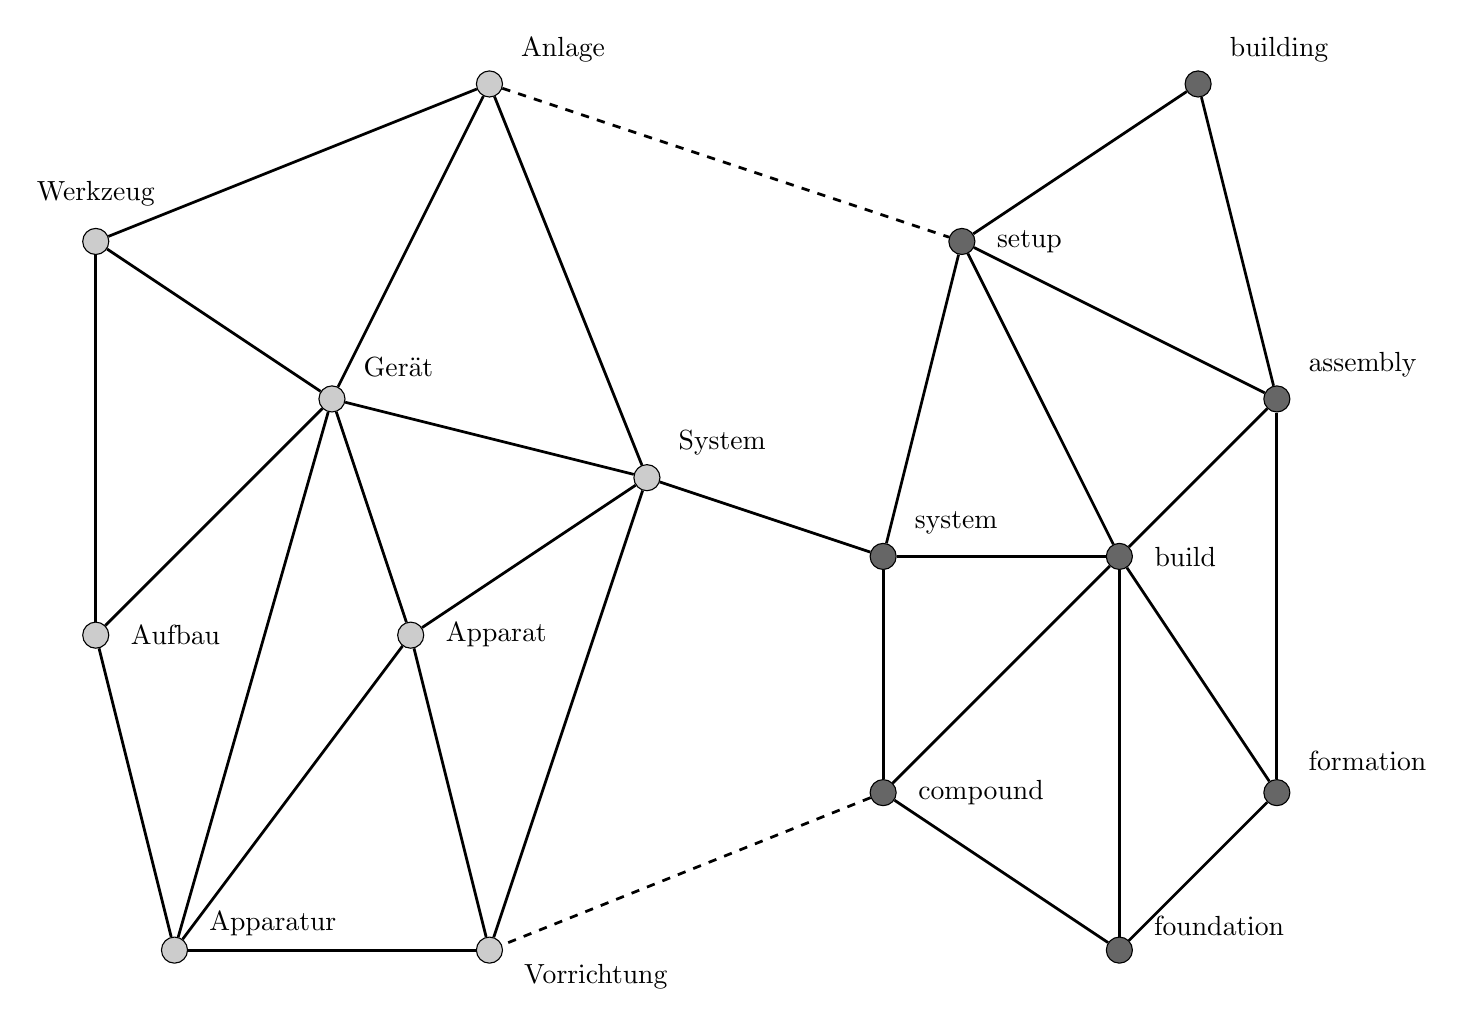
\begin{tikzpicture}
        % Styles
        \tikzstyle{line} = [draw, line width=0.1em]
        \tikzstyle{de} = [draw, circle, fill=black!20]
        \tikzstyle{en} = [draw, circle, fill=black!60]
            
        % Nodes
            \node (Werkzeug) [de,label={[label distance=0.15cm]90:Werkzeug}] at (0,10) {};  
            \node (Anlage) [de,label={[label distance=0.15cm]30:Anlage}] at (5,12) {};  
            \node (Gerät) [de,label={[label distance=0.15cm]30:Gerät}] at (3,8) {}; 
            \node (System) [de,label={[label distance=0.15cm]30:System}] at (7,7) {};   
            \node (Aufbau) [de,label={[label distance=0.15cm]0:Aufbau}] at (0,5) {};   
            \node (Apparat) [de,label={[label distance=0.15cm]0:Apparat}] at (4,5) {};  
            \node (Apparatur) [de,label={[label distance=0.15cm]10:Apparatur}] at (1,1) {}; 
            \node (Vorrichtung) [de,label={[label distance=0.15cm]-10:Vorrichtung}] at (5,1) {}; 
            
            \node (setup) [en,label={[label distance=0.15cm]0:setup}] at (11,10) {};    
            \node (building) [en,label={[label distance=0.15cm]30:building}] at (14,12){};  
            \node (assembly) [en,label={[label distance=0.15cm]30:assembly}] at (15,8){};
            \node (system) [en,label={[label distance=0.15cm]30:system}] at (10,6) {};  
            \node (build) [en,label={[label distance=0.15cm]0:build}] at (13,6) {};    
            \node (compound) [en,label={[label distance=0.15cm]0:compound}] at (10,3){};
            \node (formation) [en,label={[label distance=0.15cm]30:formation}] at (15,3) {};
            \node (foundation) [en,label={[label distance=0.15cm]10:foundation}] at (13,1){};           
        % Edges
            \path [line] (Anlage) -- (Werkzeug);
            \path [line] (Anlage) -- (Gerät);
            \path [line, dashed] (Anlage) -- (setup);
            \path [line] (Anlage) -- (System);
            \path [line] (Werkzeug) -- (Gerät);
            \path [line] (Werkzeug) -- (Aufbau);
            \path [line] (Gerät) -- (Aufbau);
            \path [line] (Gerät) -- (System);
            \path [line] (Gerät) -- (Apparat);
            \path [line] (Gerät) -- (Apparatur);
            \path [line] (Aufbau) -- (Apparatur);
            \path [line] (Apparat) -- (Apparatur);
            \path [line] (Apparat) -- (Vorrichtung);
            \path [line] (System) -- (Vorrichtung);
            \path [line] (System) -- (system);
            \path [line] (System) -- (Apparat);
            \path [line] (Apparatur) -- (Vorrichtung);
            
            \path [line] (building) -- (setup);
            \path [line] (building) -- (assembly);
            \path [line] (setup) -- (assembly);
            \path [line] (setup) -- (build);
            \path [line] (setup) -- (system);
            \path [line] (assembly) -- (formation);
            \path [line] (assembly) -- (build);
            \path [line] (build) -- (system);
            \path [line] (build) -- (formation);
            \path [line] (build) -- (foundation);
            \path [line] (build) -- (compound);
            \path [line] (system) -- (compound);
            \path [line] (compound) -- (foundation);
            \path [line, dashed] (compound) -- (Vorrichtung);
            \path [line] (formation) -- (foundation);
    \end{tikzpicture}
    }
    \caption{Mental lexicon}
    \label{oster:fig:2}
\end{figure}

\subsection{Monitoring}\label{oster:sec:1.5}
As explained above, the cognate-facilitation-effect may be an explanation for shining-through. But the \isi{source language} does not always shine through. Depending on text type and language pair, translators sometimes use fewer cognates in their translations than we see in originals \citep{Vintar2005} -- and even in translations with a tendency for shining-through, not all \isi{source language} cognates are translated by \isi{target language} cognates. Normalization in particular therefore requires a mechanism to control the production of cognates despite priming and the cognate-facilitation-effect. This mechanism might be attributed to monitoring of inner speech.

The monitoring mechanism is an important part of executive control \citep{Ganushchak2006}. It is responsible for controlling movements and \isi{speech production} in order to filter out errors and adjust behavior. Monitoring is thus not a static capacity; it is influenced by, for example, motivation \citep{Ganushchak2008}, age \citep{Wiersema2007} and \isi{time pressure} \citep{Ganushchak2006}. There is also empirical evidence that monitoring has an effect on the number of wrong motor responses a participant exhibits in an experiment -- the stronger the monitoring response, the fewer mistakes a participant makes \citep{Hajcak2003}. 

In the field of psycholinguistics, several authors assume that the monitoring mechanism also has an impact on speech output (\citealt{Aitchison2012},  \citealt{DeGroot2011}, \citealt{Levelt1999}). \citet{Levelt1999} assumes for example that speakers make many more mistakes, especially on a lexical level, if their production is not monitored. According to his theory, monitoring of the production of words takes place after the first activation of words, during inner speech. 

Verbal \isi{self-monitoring} has also been taken into consideration in the field of translation studies (e.g. \citealt{Carl2012Inside}, \citealt{TirkkonenCondit2005}, \citealt{Toury1995}). According to \citet{TirkkonenCondit2005}, translators use the easiest elements available for translation -- they transcribe the source text into the \isi{target language}. But they constantly \isi{monitor} their formulation and when they encounter problems while transcribing, they can, thanks to \isi{self-monitoring}, go back in order to find better solutions for their translation. 

In contrast to the \isi{translation process model} proposed for the purpose of this study (see \figref{oster:fig:1}), the model by Tirkkonen-Condit assumes that translators transcribe whenever possible. But as \citet{Francis2005} proved in an empirical study, translators seem to always access the conceptual level. For the purpose of this study, I will therefore not adapt Tirkkonen-Condit's model, but adjust the \isi{translation process model} presented in \figref{oster:fig:1}. A monitoring component will be added after formulation in accordance with \citet{Levelt1999} (see \figref{oster:fig:3}). I thus assume that monitoring of the production of words takes place after the first activation of words in the \isi{mental lexicon}, but that it already has an impact on the production before the first articulation occurs. 

\begin{figure}
    \resizebox{.5\textwidth}{!}{
    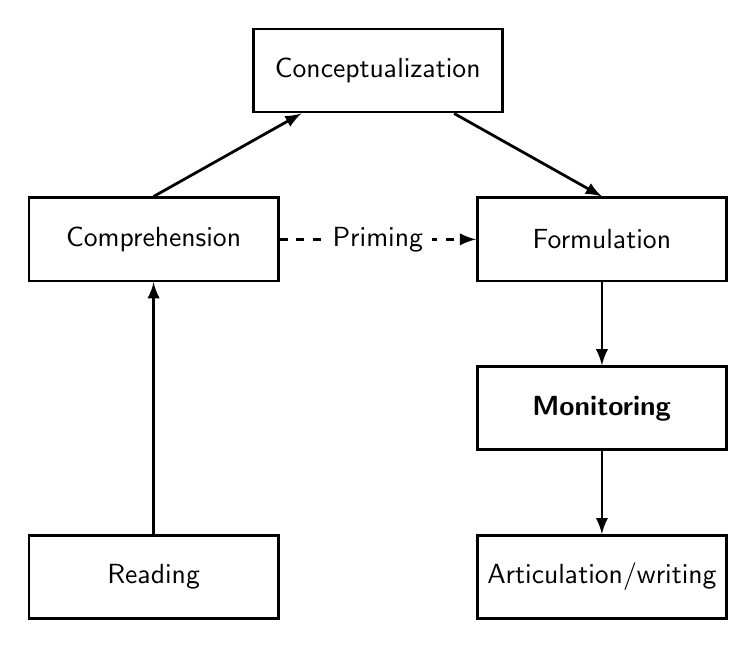
\begin{tikzpicture}
    \usetikzlibrary{shapes,arrows,positioning}
    % Styles
        \tikzstyle{block} = [rectangle, draw, fill=white, text centered, minimum height=3em, minimum width = 9em, line width = 0.1em]
        \tikzstyle{line} = [draw, -latex, line width=0.1em]
    % Place nodes
        \node [block] (conceptualization) {\sffamily{Conceptualization}};
        \node [block, below left = 3em and -1em  of conceptualization] (comprehension) {\sffamily{Comprehension}};
        \node [block, below right = 3em and -1em of conceptualization] (formulation) {\sffamily{Formulation}};
        \node [block, below = 3em of formulation] (monitoring) {\sffamily{\textbf{Monitoring}}};
        \node [block, below = 3em of monitoring] (articulation) {\sffamily{Articulation/writing}};
        \node [block, below = 9.1em of comprehension] (reading) {\sffamily{Reading}};
    % Draw edges
        \path [line] (reading) -- (comprehension);
        \path [line] (comprehension.north) -- (conceptualization);
        \path [line] (conceptualization) -- (formulation.north);
        \path [line] (formulation) -- (monitoring);
        \path [line] (monitoring) -- (articulation);
    % Label
        \draw[line, dashed] (comprehension) -- (formulation) node [midway, fill=white] {\sffamily{Priming}};
    \end{tikzpicture}
    }
 	\caption{Translation process with monitoring}
 	\label{oster:fig:3}
\end{figure}

There has not yet been any evidence that \isi{self-monitoring} has an influence on the production of cognates, which are not necessarily real mistakes. A study by \citet{Kussmaul1989}, however, can provide a first hint that the number of cognates is indeed reduced by the monitoring mechanism. Kußmaul discovered that translation students often use cognates in their translations first, but then decide to replace them with non-cognates. He calls this phenomenon \textit{Interferenzphobie} (fear of interferences). Kußmaul focused on the best way to verbalize a concept and not on quantitative characteristics of a text, which is what I investigated in the present study. However, Kußmaul's study provides us with sufficient reasons to take \isi{self-monitoring} into consideration when investigating mechanisms leading to normalization.

How can \isi{self-monitoring} be investigated during translation of whole texts? It is widely accepted that the oral and the written production mode mainly differ in the degree of monitoring -- the capacity to \isi{monitor} is stronger in written production than in \isi{oral production} \citep{Treiman2003}. This could be due to the time available for production. As \citet{Ganushchak2006} showed, the more time participants have to answer, the stronger their monitoring is. And more time is usually available for writing than for speaking tasks. In this study, I applied this mechanism and compared oral and written translations in regard to the translation of cognates. The hypothesis I tested is that \isi{self-monitoring} has an influence on the number of cognates in translations and that written translations therefore contain fewer cognates than oral translations.

\section{Method}\label{oster:sec:2}

The only difference between oral and written production regarding the different steps of the language processing model and the processing of words is the degree of monitoring. It is lower for the oral than for the written production mode \citep{Treiman2003}. In order to investigate the influence of \isi{self-monitoring} on the number of cognates in translations, I compared written and oral translations.

\subsection{Experiment 1}\label{oster:sec:2.1}
In a first experiment, translation students translated a written text with a high cognate-density from English into \ili{German}. Although this language pair shows a tendency towards shining-through \citep{Vintar2005}, not all \isi{source language} cognates are translated by using \isi{target language} cognates. The control mechanism must therefore also be present when working with these two languages. The translations from this experiment were later compared to oral translations. 

The source text was taken from the American news platform \href{http://foxnews.com}{foxnews.com}. The text on foreign affairs was presented in American English; the topic was also being discussed in the \ili{German} media at the time of the experiment. The text was slightly modified in order to fit the requirements of the study: the participants had to translate the text without any translation aids and in a reasonable timeframe. Terms that were deemed too difficult for this purpose were replaced by easier expressions (e.g. \textit{threatened to retaliate} by \textit{threatened revenge}). The text was also shortened to enable a reduced translation time and to increase the \isi{cognate} density. For this purpose, direct citations of an interview conducted for the article were removed. These citations were also discussed again in the text and were therefore not essential in order to understand the text. The final version of the source text was 190 words long and contained 21 English-\ili{German} cognates. The cognates were defined as words which shared form and approximate meaning in English and \ili{German}. Words, which were not found in the \ili{German} dictionary \textit{Duden}, were defined as borrowings and thus not analyzed for the purpose of this study. I did not distinguish between true cognates and false friends \citep{Stamenov2010}, since this study concentrated on form and not on meaning. 

A group of 39 participants performed a written translation at the Faculty of Translation Studies, Linguistics and Cultural Studies in Germersheim. The participants were translation students who already had some experience in translating; they were in their 2\textsuperscript{nd} year or higher. English was their first or second foreign language. They were all \ili{German} native speakers. The experiment was carried out in the course of a lecture the participants attended, but they participated voluntarily and could withdraw from the experiment at any time. They were informed that their translations would be treated anonymously and would not be evaluated except for the purpose of the present study. 

The participants were instructed to translate the text without making any changes once it was written down. They were not allowed to use any translation aids such as dictionaries or online resources. They were told that the translation should not take more than 30 minutes, but no definite limits were communicated and every participant was able to finish the translation when he or she wanted.

\subsection{Experiment 2}\label{oster:sec:2.2}
In a second experiment, a group of 18 participants completed an oral translation. These texts were then compared to the written translations in experiment~1. 

\newpage
The participants were chosen under the same conditions as in experiment~1. They read the written source text of experiment~1 and spoke the translation. The experiment was performed in private. The participants used their own computers and audio registration software to record their voice: \citet{Whyatt2010} argues that self-recording causes fewer interferences and leads to a more natural setting, which was also the case in experiment~1. The participants were asked to verbalize every word that crossed their minds, in order to reveal further monitoring steps before the final version was chosen. As in experiment~1, the participants were asked not to use any translation aids.

\section{Results}\label{oster:sec:3}
The written and oral translations were analyzed with a focus on the translation of the previously defined cognates and on a qualitative and a quantitative level. For the quantitative analysis, the number of source text cognates translated into \isi{target language} cognates was counted in both the oral and written translations. For the qualitative analysis, I investigated how the translators dealt with cognates during the oral translation in experiment~2.

\subsection{Quantitative results}\label{oster:sec:3.1}
Since not all of the participants verbalized all source text cognates and sometimes left out phrases, sentences or whole paragraphs, I computed the percentage of cognates translated with cognates compared to all cognates translated. Thereby, the non-verbalized cognates were not taken into consideration and incomplete translations could be considered for the analysis as well. Cognate production was analyzed in three different phases and modes (see \figref{oster:fig:4}): the written production of experiment~1, the first production of experiment~2 (\isi{oral production}) and the final production of experiment~2. The number of cognates was lower in the final \isi{oral production} (60.56~\%) compared to the first \isi{oral production} (65.53~\%) and the lowest number of cognates was found in the written translations (56.56~\%).

For the statistical analysis, a Wilcoxon Signed-Rank Test was performed on the results of the two dependent samples of the \isi{oral production} phases. The number of cognates was significantly lower in the final \isi{oral production} phase (M~=~60.56, SD~=~7.41) compared to the first \isi{oral production} phase (M~=~65.53, SD~=~9.19); V~=~90.5, p~=~.009.

A Wilcoxon-Mann-Whitney test was performed on the independent samples of the final version of experiment~2 and the written production. The number of cognates was significantly lower in the written production (M~=~56.56, SD~=~9.19) compared to the final \isi{oral production} (M~=~60.56, SD~=~7.41); W=~479, p=~.014.

\begin{figure}
	
    % barplot command seems broken
  	%\barplot{}{\%}{First \isi{oral production}, Final \isi{oral production}, Written production}{
   	%  	(First \isi{oral production},65.53)
    % 	(Final \isi{oral production},60.56)
    %  	(Written production,56.56)
	%}
 	\includegraphics[width=.5\textwidth]{figures/oster/figure4.pdf}
 	\caption{The number of cognates in different translation modes and phases\protect\footnotemark}
 	\label{oster:fig:4}
\end{figure}
% TODO: Is on wrong page
\footnotetext{{See \sectref{oster:sec:4} for discussion.}}

\subsection{Qualitative results}\label{oster:sec:3.2}
In addition to the quantitative analysis, a qualitative analysis was performed on the translations in experiment~2. I investigated how the participants dealt with the cognates during verbalization of their translation; whether they directly chose one word as an adequate translation or whether they first chose one expression which was then replaced by another word they thought was better. 

Twelve of the 18 participants chose a \isi{target language} \isi{cognate} at least once first in order to verbalize the meaning of a \isi{cognate} in the source text (ST) before replacing it with a non-\isi{cognate} in the target text (TT). This replacement was performed in 26 cases in total. 

Examples \ref{oster:ex:1} to \ref{oster:ex:3} show how these cognate-non-\isi{cognate} replacements were performed during the verbalization process. In \exref{oster:ex:1}, the participant initially decided to translate the English word \textit{meeting} with the \ili{German} \isi{cognate} \textit{Meeting}, but then chose to replace it with \textit{Versammlung} and finally chose \textit{Konferenz} as the best translation. This replacement of a \isi{cognate} by a non-\isi{cognate} can also be seen in \exref{oster:ex:2}. The participant first translated the English word \textit{guarantees} with the \ili{German} \isi{cognate} \textit{Garantien}, but then decided to replace it with \textit{Zusicherungen}. \exref{oster:ex:3} shows how the participant gradually moved away from the \isi{cognate}. He first translated \textit{undermine} with \textit{unterminieren}, then changed it to \textit{unterwandern} which still shares some formal aspects, the prefix, with the English word \textit{undermine}. The participant finally used a word that does not share any formal aspects with the \isi{cognate}, by using the \ili{German} word \textit{einzuschränken}.

\ea%1
    \label{oster:ex:1}
    \glt \textbf{ST}: Medvedev told in a meeting [\ldots]
    \glt \textbf{TT}: Medwedew sagte in einem Meeting \ldots sagte in einer Versammlung \ldots in einer Konferenz [\ldots]
    \z

\ea%2
    \label{oster:ex:2}
    \glt \textbf{ST}: [\ldots] Medvedev has sought guarantees from the U.S. [\ldots]
    \glt \textbf{TT}: [\ldots] wollte Medwedew Garantien \ldots Zusicherungen \ldots eine Zusicherung von der US-amerikanischen Regierung haben [\ldots]
\z

\ea%3
    \label{oster:ex:3}
    \glt \textbf{ST}: [\ldots] powerful enough to undermine Russia's Power.
    \glt \textbf{TT}: [\ldots] mächtig genug sein wird, um Russlands Macht zu unterminieren \ldots zu unterwandern \ldots um Russlands eigene Macht einzuschränken. 
\z

Changes after the first verbalization were not always cognate-non-\isi{cognate} replacements. In one instance, three participants first chose a non-\isi{cognate} and then replaced it with a \isi{cognate}. One of these non-cognate-\isi{cognate} replacements can be seen in \exref{oster:ex:4}

\ea%4
    \label{oster:ex:4}
    \glt \textbf{ST}: Without a NATO-Russia cooperation \textit{deal} [\ldots]
    \glt \textbf{TT}: Ohne eine Absprache \ldots einen \textit{Deal} zwischen der NATO und Russland [\ldots]
\z

Although some participants replaced non-cognates with cognates, the cognate-non-\isi{cognate} replacements outweigh reverse changes. The qualitative analysis thus supports the quantitative results. Cognates are often the  words initially chosen for translation. But when translators have more time available, they replace some cognates with  non-cognates.

\section{Discussion}\label{oster:sec:4}
The quantitative analysis of experiments~1 and 2 showed that the number of cognates decreased with the time available for production. During the first production during oral translation, participants used more cognates than during the final production phase which still contained more cognates than the written production. Since the difference in \isi{production time} \citep{Ganushchak2006}, as well as the different production modes \citep{Treiman2003} can be linked to stronger monitoring, the decreased number of cognates can be explained by stronger \isi{self-monitoring} during  production. 

This interpretation is supported by the qualitative analysis of experiment~2. In most cases, changes that were made to the translation of cognates were cognate-non-\isi{cognate} replacements. Although non-cognates were replaced by cognates in some cases, the number of cognate-non-\isi{cognate} replacements outweighs the number of non-cognate-\isi{cognate} replacements: difficulties in verbalizing every word and thought that comes to mind could have caused the few non-cognate-\isi{cognate} replacements. The cognate-non-\isi{cognate} replacements thus suggest that it might be easier for the translator to translate source text cognates with \isi{target language} cognates. This can be explained by the cognate-facilitation-effect and priming. The translator then tries to control production by filtering out the cognates. These results thus support the hypothesis that cognates are indeed activated first and then filtered out with the help of \isi{self-monitoring}.

The aim of this study was to investigate the mechanisms which lead to shining-through and normalization. Psycholinguistic literature shows that the structure and functions of the \isi{mental lexicon} can explain facilitated access to cognates compared to non-cognates. The cognate-facilitation-effect and priming can therefore explain the shining-through effect. The hypothesis tested in the present study was therefore that shining-through occurs naturally but that cognates are filtered out by \isi{self-monitoring}. This was investigated by comparing written and oral translations of a written English text into \ili{German} by translation students due to the differences in magnitude in terms of the monitoring mechanism. The results support the hypothesis that \isi{self-monitoring} after the first activation of words has an impact on the number of cognates in translations and enables translators to control their production despite the cognate-facilitation-effect. 

I may thus conclude that verbal \isi{self-monitoring} not only has an effect on the number of real mistakes as \citet{Levelt1999} suggested but also on minor tendencies in the text such as the number of cognates. Verbal \isi{self-monitoring} might therefore be an important factor regarding normalization and play an important part in the \isi{translation process}. The results of the present study support recent \isi{translation process} models (e.g. \citealt{TirkkonenCondit2005}) and could lead to the conclusion that verbal \isi{self-monitoring} after the first activation of words, but before articulation and writing, should be taken into consideration when investigating and modeling the \isi{translation process}.

\newpage
\sloppy
\printbibliography[heading=subbibliography,notkeyword=this]
\end{document}

% \sffamily
% @book{Aitchison2012,
% 	address = {Oxford},
% 	author = {Aitchison, J.},
% 	publisher = {Wiley-Blackwell},
% 	title = {\textit{Words in the mind: an introduction to the mental lexicon}},
% 	year = {2012}
% }
% 
% \sffamily
% Baker, M. 1996. Corpus-based translation studies: The challenges that lie ahead. \textit{Terminology, LSP and Translation: Studies in language engineering in honour of Juan C. Sager}, H. Somers (Ed.), 175-186. Amsterdam/Philadelphia: John Benjamins.
% 
% \sffamily
% Becher, V.; House, J.; Kranich, S. 2009. Convergence and divergence of communicative norms through language contact in translations. \textit{Convergence and divergence in language contact situations}, K. Braunmüller; J. House (Eds.), 125-152. Amsterdam/Philadelphia: John Benjamins.
% 
% \sffamily
% @article{Carl2012,
% 	author = {Carl, M.; Dragsted, B},
% 	journal = {\textit{Translation: Corpora, Computation, Cognition}},
% 	number = {1},
% 	pages = {127-145},
% 	title = {Inside the Monitor Model: Processes of Default and Challenged Translation Production},
% 	volume = {2},
% 	year = {2012}
% }
% 
% \sffamily
% @article{Christoffels2006,
% 	author = {Christoffels, I.K.; De Groot, A.M.B.; Kroll, J.F},
% 	journal = {\textit{Journal of Memory and Language}},
% 	pages = {324-345},
% 	title = {Memory and language skills in simultaneous interpreters: The role of expertise and language proficiency},
% 	volume = {54},
% 	year = {2006}
% }
% 
% \sffamily
% @article{Christoffels2007,
% 	author = {Christoffels, I.K.; Firk, C.; Schiller, N.O},
% 	journal = {\textit{Brain and Research}},
% 	pages = {192-208},
% 	title = {Bilingual language control: An event-related brain potential study},
% 	volume = {1147},
% 	year = {2007}
% }
% 
% \sffamily
% @article{Costa1999,
% 	author = {Costa, A.; Caramazza, A},
% 	journal = {\textit{Bilingualism: Language and Cognition}},
% 	number = {3},
% 	pages = {231-244},
% 	title = {Is lexical selection in bilingual \isi{speech production} language specific? Further evidence from \ili{Spanish}-English and English-\ili{Spanish} bilinguals},
% 	volume = {2},
% 	year = {1999}
% }
% 
% \sffamily
% @article{Costa2000,
% 	author = {Costa, A.; Caramazza, A., Sebastiàn-Gallés, N},
% 	journal = {\textit{Journal of Experimental Psychology: Learning, Memory and Cognition}},
% 	pages = {1283-1296},
% 	title = {The Cognate Facilitation Effect: Implications for Models of Lexical Access},
% 	volume = {26},
% 	year = {2000}
% }
% 
% \sffamily
% @article{Costa2005,
% 	author = {Costa, A.; Santesteban, M.; Caño; A},
% 	journal = {\textit{Brain and Language}},
% 	pages = {94-103},
% 	title = {On the facilitatory effects of \isi{cognate} words in bilingual speech production},
% 	volume = {94},
% 	year = {2005}
% }
% 
% \sffamily
% De Bot, K.; Schreuder, R. 1993. Word Production and the Bilingual Lexicon. \textit{The Bilingual Lexicon}, R. Schreuder; B. Weltens (Eds.), 191- 214. Amsterdam/Philadelphia: John Benjamins.
% 
% \sffamily
% @book{De2011,
% 	address = {New York},
% 	author = {De Groot, A.M.B.},
% 	publisher = {Psychology Press},
% 	title = {\textit{Language and Cognition in Bilinguals and Multilinguals. An Introduction}},
% 	year = {2011}
% }
% 
% \sffamily
% @article{Dell1986,
% 	author = {Dell, G.S},
% 	journal = {\textit{Psychological Review}},
% 	number = {3},
% 	pages = {283-321},
% 	title = {A Spreading-Activation Theory of Retrieval in Sentence Production},
% 	volume = {93},
% 	year = {1986}
% }
% 
% \sffamily
% @article{Dell1992,
% 	author = {Dell, G.S.; O’Seaghdha, P.G},
% 	journal = {\textit{Cognition}},
% 	pages = {287-314},
% 	title = {Stages of lexical access in language production},
% 	volume = {42},
% 	year = {1992}
% }
% 
% \sffamily
% @article{Francis2005,
% 	author = {Francis, W.S.; Gallard, S.L.K},
% 	journal = {\textit{Psychonomic Bulletin \& Review}},
% 	number = {16},
% 	pages = {1082-1088},
% 	title = {Concept \isi{mediation} in trilingual translation: Evidence from response times and repetition priming patterns},
% 	volume = {12},
% 	year = {2005}
% }
% 
% \sffamily
% @article{Ganushchak2006,
% 	author = {Ganushchak, L.Y.; Schiller, N.O},
% 	journal = {\textit{Brain Research}},
% 	pages = {104-115},
% 	title = {Effects of \isi{time pressure} on verbal \isi{self-monitoring}: An ERP study},
% 	volume = {1125},
% 	year = {2006}
% }
% 
% \sffamily
% @article{Ganushchak2008,
% 	author = {Ganushchak, L.Y.; Schiller, N.O},
% 	journal = {\textit{NeuroImage}},
% 	pages = {395-405},
% 	title = {Motivation and semantic context affect brain error-monitoring activity: An event-related brain potentials study},
% 	volume = {39},
% 	year = {2008}
% }
% 
% \sffamily
% @article{Hajcak2003,
% 	author = {Hajcak, G.; McDonald, N.; Simons, R.F},
% 	journal = {\textit{Psychophysiology}},
% 	pages = {895-903},
% 	title = {To err is automatic. Error-related brain potentials, ANS activity, and post error-compensatory behavior},
% 	volume = {40},
% 	year = {2003}
% }
% 
% \sffamily
% Hansen-Schirra, S. 2012. What do these results suggest? Crosslinguistic variation of non-agentive subjects and the role of translation. \textit{Anglistentag-Proceedings}, C. Schubert; U. Gut (Eds.).
% 
% \sffamily
% @book{Hönig1997,
% 	address = {Tübingen},
% 	author = {Hönig, H.G.},
% 	publisher = {Narr},
% 	title = {\textit{Konstruktives Übersetzen}},
% 	year = {1997}
% }
% 
% \sffamily
% @article{Ibáñez2010,
% 	author = {Ibáñez, A.J.; Macizo, P.; Bajo, M.T},
% 	journal = {\textit{Acta Psychologica}},
% 	pages = {257-266},
% 	title = {Language access and language selection in professional translators},
% 	volume = {135},
% 	year = {2010}
% }
% 
% \sffamily
% @book{Kiraly1995,
% 	address = {Kent},
% 	author = {Kiraly, D.C.},
% 	publisher = {The Kent State University Press},
% 	title = {\textit{Pathways to Translation: Pedagogy and Process}},
% 	year = {1995}
% }
% 
% \sffamily
% @book{Krings1986,
% 	address = {Tübingen},
% 	author = {Krings, H.P.},
% 	publisher = {Narr},
% 	title = {\textit{Was in den Köpfen von Übersetzern vorgeht: Eine empirische Untersuchung zur Struktur des Übersetzungsprozessses an fortgeschrittenen Französischlernern}},
% 	year = {1986}
% }
% 
% \sffamily
% @book{Kautz2000,
% 	address = {München},
% 	author = {Kautz, U.},
% 	publisher = {Iudicium},
% 	title = {\textit{Handbuch Didaktik des Übersetzens und Dolmetschens}},
% 	year = {2000}
% }
% 
% \sffamily
% Kußmaul, P. 1989. Interferenzen im Übersetzungsprozeß – Diagnose und Therapie. \textit{Interferenz in der Translation}, H. Schmidt (Ed.), 19-28. Leipzig: VEB Enzyklopädie.
% 
% \sffamily
% @book{Levelt1989,
% 	address = {Cambridge/London},
% 	author = {Levelt, W.J.M.},
% 	publisher = {MIT Press},
% 	title = {\textit{Speaking: From Intention to Articulation}},
% 	year = {1989}
% }
% 
% \sffamily
% Levelt, W.J.M. 1999. Producing spoken language: a blueprint of the speaker. \textit{The Neurocognition of Language}, C.M. Brown; P. Hagoort (Eds.), 83-122. New York: Oxford University Press.
% 
% \sffamily
% @book{Paradis2004,
% 	address = {Amsterdam},
% 	author = {Paradis, M.},
% 	publisher = {John Benjamins},
% 	title = {\textit{A Neurolinguistic Theory of Bilingualism}},
% 	year = {2004}
% }
% 
% \sffamily
% @book{Plieger2006,
% 	address = {Berlin},
% 	author = {Plieger, P.},
% 	publisher = {Lit},
% 	title = {\textit{Struktur und Erwerb des bilingualen Lexikons}},
% 	year = {2006}
% }
% 
% \sffamily
% Stamenov, I.M.; Gerganov, A.; Popivanov, I.D. 2010. Prompting cognates in the bilingual lexicon: Optimizing access during translation.\textit{Translation and Cognition}. G.M. Shreve; E. Angelone (Eds.), 323-348. Amsterdam: John Benjamins.
% 
% \sffamily
% @book{Steiner2001,
% 	address = {Oslo},
% 	author = {Steiner, E.},
% 	publisher = {University of Oslo},
% 	title = {Translations English-\ili{German}: investigating the relative importance of systemic contrasts and of the text-type “translation”. \textit{SPRIKreport no. 7. Reports from the project “Languages in Contrast”}},
% 	year = {2001}
% }
% 
% \sffamily
% @book{Teich2003,
% 	address = {Berlin},
% 	author = {Teich, E.},
% 	publisher = {Mouton de Gruyter},
% 	title = {\textit{Cross-Linguistic Variation in System and Text: A Methodology for the Investigation of Translations and Comparable Texts}},
% 	year = {2003}
% }
% 
% \sffamily
% @article{Tirkkonen-Condit2005,
% 	author = {Tirkkonen-Condit, S},
% 	journal = {\textit{Translators' Journal}},
% 	number = {2},
% 	pages = {405-414},
% 	title = {The Monitor Model Revisited: Evidence from Process Research},
% 	volume = {50},
% 	year = {2005}
% }
% 
% \sffamily
% @book{Toury1995,
% 	address = {Amsterdam/Philadelphia},
% 	author = {Toury, Gideon.},
% 	publisher = {John Benjamins},
% 	title = {\textit{Descriptive Translation Studies and Beyond}},
% 	year = {1995}
% }
% 
% \sffamily
% Treiman, R.; Clifton, C.Jr; Meyer, A.S.; Wurm, L.H. 2003. Language Comprehension and Production. \textit{Comprehensive Handbook of Psychology, Volume 4: Experimental Psychology}, A.F. Healy; R.W. Proctor. (Eds.), 527-548. New York: Wiley.
% 
% \sffamily
% Vintar, S.; Hansen-Schirra, S. 2005. Cognates. free rides, false friends or stylistic devices?: a corpus-based comparative study. \textit{Meaningful texts: the extraction of semantic information from monolingual and multilingual corpora, (Research in corpus and discourse)}. G. Barnbrook; P. Danielsson; M. Mahlberg (Eds.), 208-221. London/New York: Continuum.
% 
% \sffamily
% Whyatt, B. 2010. Bilingual Language Control in Translation Tasks: A TAP Study into Mental Effort Management by Inexperienced Translators. \textit{Neurolinguistic and Psycholinguistic Perspectives on SLA}. J. Arabski (Ed.), 79-92. Bristol/Buffalo/Toronto: Multilingual Matters.
% 
% \sffamily
% @article{Wiersema2007,
% 	author = {Wiersema, J.R.; van der Meere, J.J.; Roeyers, H},
% 	journal = {Neuropsychologia},
% 	pages = {1649-1657},
% 	title = {Developmental changes in error monitoring: An event related potential study},
% 	volume = {45},
% 	year = {2007}
% }
